The steps above ensured the establishment of the physical, data link, network, and transport layers, drawing up the foundation for the application layer, featuring the actual implementation of the \pol{} protocol. In this section, we provide a description of the protocol setup, including the reasoning and choice for the Blockchain framework to use. The processes of proof generation and verification are also detailed.

\subsubsection{Practical Permissionless Consensus} \label{sec:pol-implementation:practical-permissionless-consensus}

The outline provided in Section~\ref{sec:protocol-fundamentals-clock} identified the need for a clock synchronization mechanism that would finally enable spatio-temporal soundness. Space synchrony is achieved with the assumptions around the short-ranged communication means. Time synchrony, on the other hand, is achieved with a clock synchronization mechanism. The hypothesis involved the employment of a permissionless consensus protocol to establish zone-relative time consciousness, but with the added benefit of providing strongly consistent serialization of transactions and total order of multidimensional events, instead of simply counting time in a unidimensional manner, via a plain clock synchronization protocol. The practicalities of employing a permissionless consensus mechanism involved the experimentation with a blockchain framework, the deployment of an interacting client, and the setup of the network.

The beginning of the exploration process included the prototyping of an ad hoc Proof-of-Work based consensus protocol, to assess the feasibility of the hypothesis. This work was part of the 2022 Fall Semester's edition of the Distributed Systems seminar, where an analytical approach was taken to survey multiple permissionless consensus mechanisms, pointing out the challenges of porting such protocols to resource constrained environments\footnote{\url{https://github.com/edurbrito/dist-sys-seminar}}. The results of the experiment were sufficiently encouraging to warrant the development or choice of a more robust and scalable implementation. Multiple open source projects were considered, and the ultimate decision relied on Ethereum and its flexible tooling for creating private networks\footnote{\url{https://geth.ethereum.org/docs/fundamentals/private-network}}. Initially, the successful attempts at interacting with Ethereum concealed a handful of problems that would be later uncovered. The smart contracts' functionality, for instance, was presenting issues at the execution and output conversion. The problems were ultimately traced back to the use of a different version of the contract's compiler, which was not compatible with the version of the client used. Some of the issues persisted, which led us to ask for help from the Ethereum community, in GitHub\footnote{\url{https://github.com/ethereum/go-ethereum/issues/27009}}, StackExchange, and other forums. We have eventually solved the problem, with a custom compilation of the software, and have successfully blended its official client implementation, \emph{geth}, into the OpenWrt image.

The prerequisites for the establishment of an ad hoc Ethereum network expect first the configuration of a \emph{Genesis} file and a local data directory, to set the initial state of the network and progressively save the history, as the blocks get mined. Configuring the genesis block resorts, as well, to the choice of a consensus protocol. The geth client supports two main consensus protocols, a Proof-of-Work (PoW) and a Proof-of-Authority (PoA) based mechanism. Both protocols were tried out, but PoA was ultimately chosen for carrying out the remaining tests, since it offered a more controlled environment for the flexible adjustment of multiple parameters, like the block time. A more thorough analysis of the PoW and PoA protocols, as well as trade-offs and performance comparisons, are left for future work. The PoA protocol relies on a list of authorized signers, which are allowed to mine blocks \cite{clique-eth}. The signers' list is defined in the genesis block, and the private key of each signer is used to sign the blocks. We have automated the key pair generation at startup and developed multiple utility programs to facilitate the deployment of the nodes and the execution of the protocol. These custom tools were written in Golang and compiled for the target platform, to be used as part of the OpenWrt image, serving also as demonstration of the feasibility of the process of embedding custom software into the system. These command-line programs can be found under the "proof-of-concept/src/geth-utils" directory. Among other tasks, they automate the initialization of the blockchain nodes, via the genesis file, and the establishment of the network, via the discovery of bootnodes and connection of new peers. Each node exposes the necessary API endpoints to allow for the interaction with the rest of the protocol participants. Network rules were also configured to restrict the communication to the zone subnet, as well as a caching policy to avoid unnecessary resource consumption. Everything was accomplished with the help of the Ethereum geth client, and the final blockchain network arrangement is illustrated in Figure~\ref{fig:pol-implementation:blockchain-network}.

\begin{figure}[h!]
    \begin{center}
    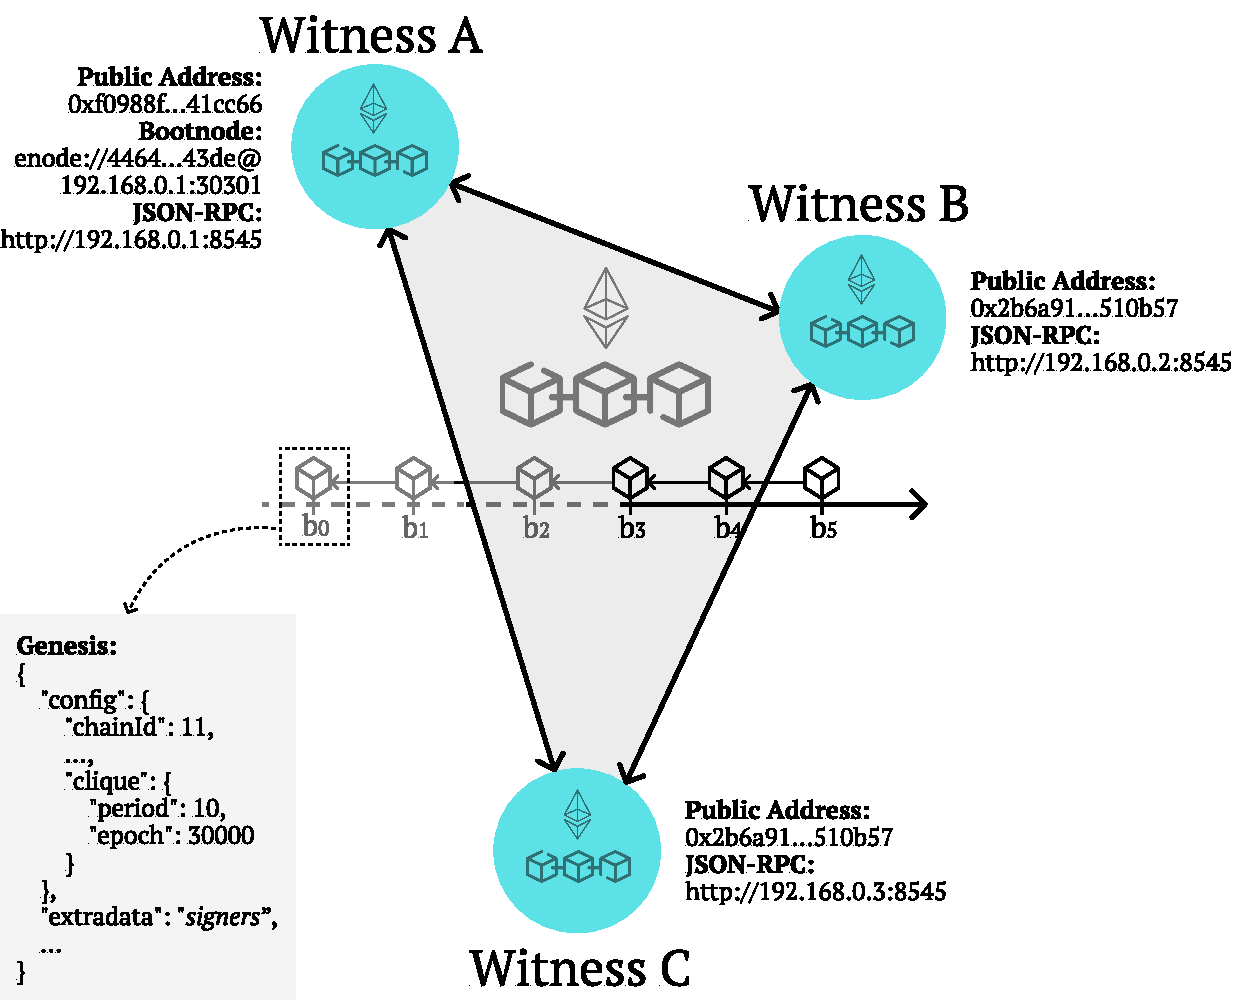
\includegraphics[width=0.75\textwidth]{proof-of-concept-blockchain.pdf}
    \caption{The Ethereum blockchain network setup, featuring a Proof-of-Authority consensus protocol with a block time of 10 seconds.}
    \label{fig:pol-implementation:blockchain-network}
    \end{center}
\end{figure}

\subsubsection{Proof Generation and Verification} \label{sec:pol-implementation:proof-generation-verification}

Guaranteed the establishment of a permissionless consensus mechanism, the witnesses are finally synchronized in time. The prover can now take advantage of this synchrony to request the generation of a \pol{} certificate. To accomplish such task, the prover instance, which is also part of the mesh network communication channel and has been assigned an IP address in the same subnet, needs to interact with the running blockchain and follow the protocol specified in Section~\ref{sec:protocol-fundamentals-rel-pol}. 

The automation of the prover process was also achieved with the help of a Golang utility program, found under the "proof-of-concept/src/geth-utils" directory. A random witness is first chosen and inquired about the most recent block. After that, a transaction is assembled, signed, and submitted. All the requests are accomplished via the JSON-RPC API exposed by the geth client running in the witnesses' machines. The transaction is then broadcasted to the network and the prover waits for it to be included in a block. Once the transaction is confirmed, the prover can verify its validity. If valid, it can finally request the block signatures from the witnesses. The transaction validation process may be automated via the deployment of a smart contract in the network, decentralizing and automating the procedure. An example of a smart contract, located in the "proof-of-concept/src/block-verifier" directory, was also developed and successfully deployed. The contract was written in Solidity\footnote{\url{https://docs.soliditylang.org/en/v0.8.19/}}, compiled to the Ethereum Virtual Machine (EVM) bytecode, and included in the genesis file. It compares the input hash, submitted by the prover, with the hash of the last block in the network. The contract is invoked via a typical blockchain transaction, and returns a boolean value, indicating whether the transaction is valid or not, automating the validation process that would otherwise be performed manually, by either the prover or the verifier. This approach serves as demonstration of the feasibility of the deployment of smart contracts in the zone's blockchain. More sophisticated contracts can be developed and deployed according to application needs, expanding the possibilities of the protocol and its use cases for providing decentralized and zone-relative location services (see Section~\ref{sec:protocol-fundamentals-clock}). Furthermore, the success of the proof generation process is dependent on the adjustment of the block time, which is a parameter that can be configured in the chosen PoA protocol. We have set the block time $T$ to 10 seconds, in our current implementation. Similar to the time-limited approach presented by Nosouhi et al. \cite{nosouhi2020blockchain}, the block interval serves the purpose of preventing proxy or wormhole attacks, as depicted in Figure~\ref{fig:pol-implementation:overview-proxy-wormhole}, shortening the chances for an adversary that is synchronized with the witnesses to interact with a remote prover and still be able to generate a spatio-temporally sound \pol{} certificate. This time interval should be planned and adjusted according to the application needs and the desired levels of security.

\begin{figure}[h!]
    \begin{center}
    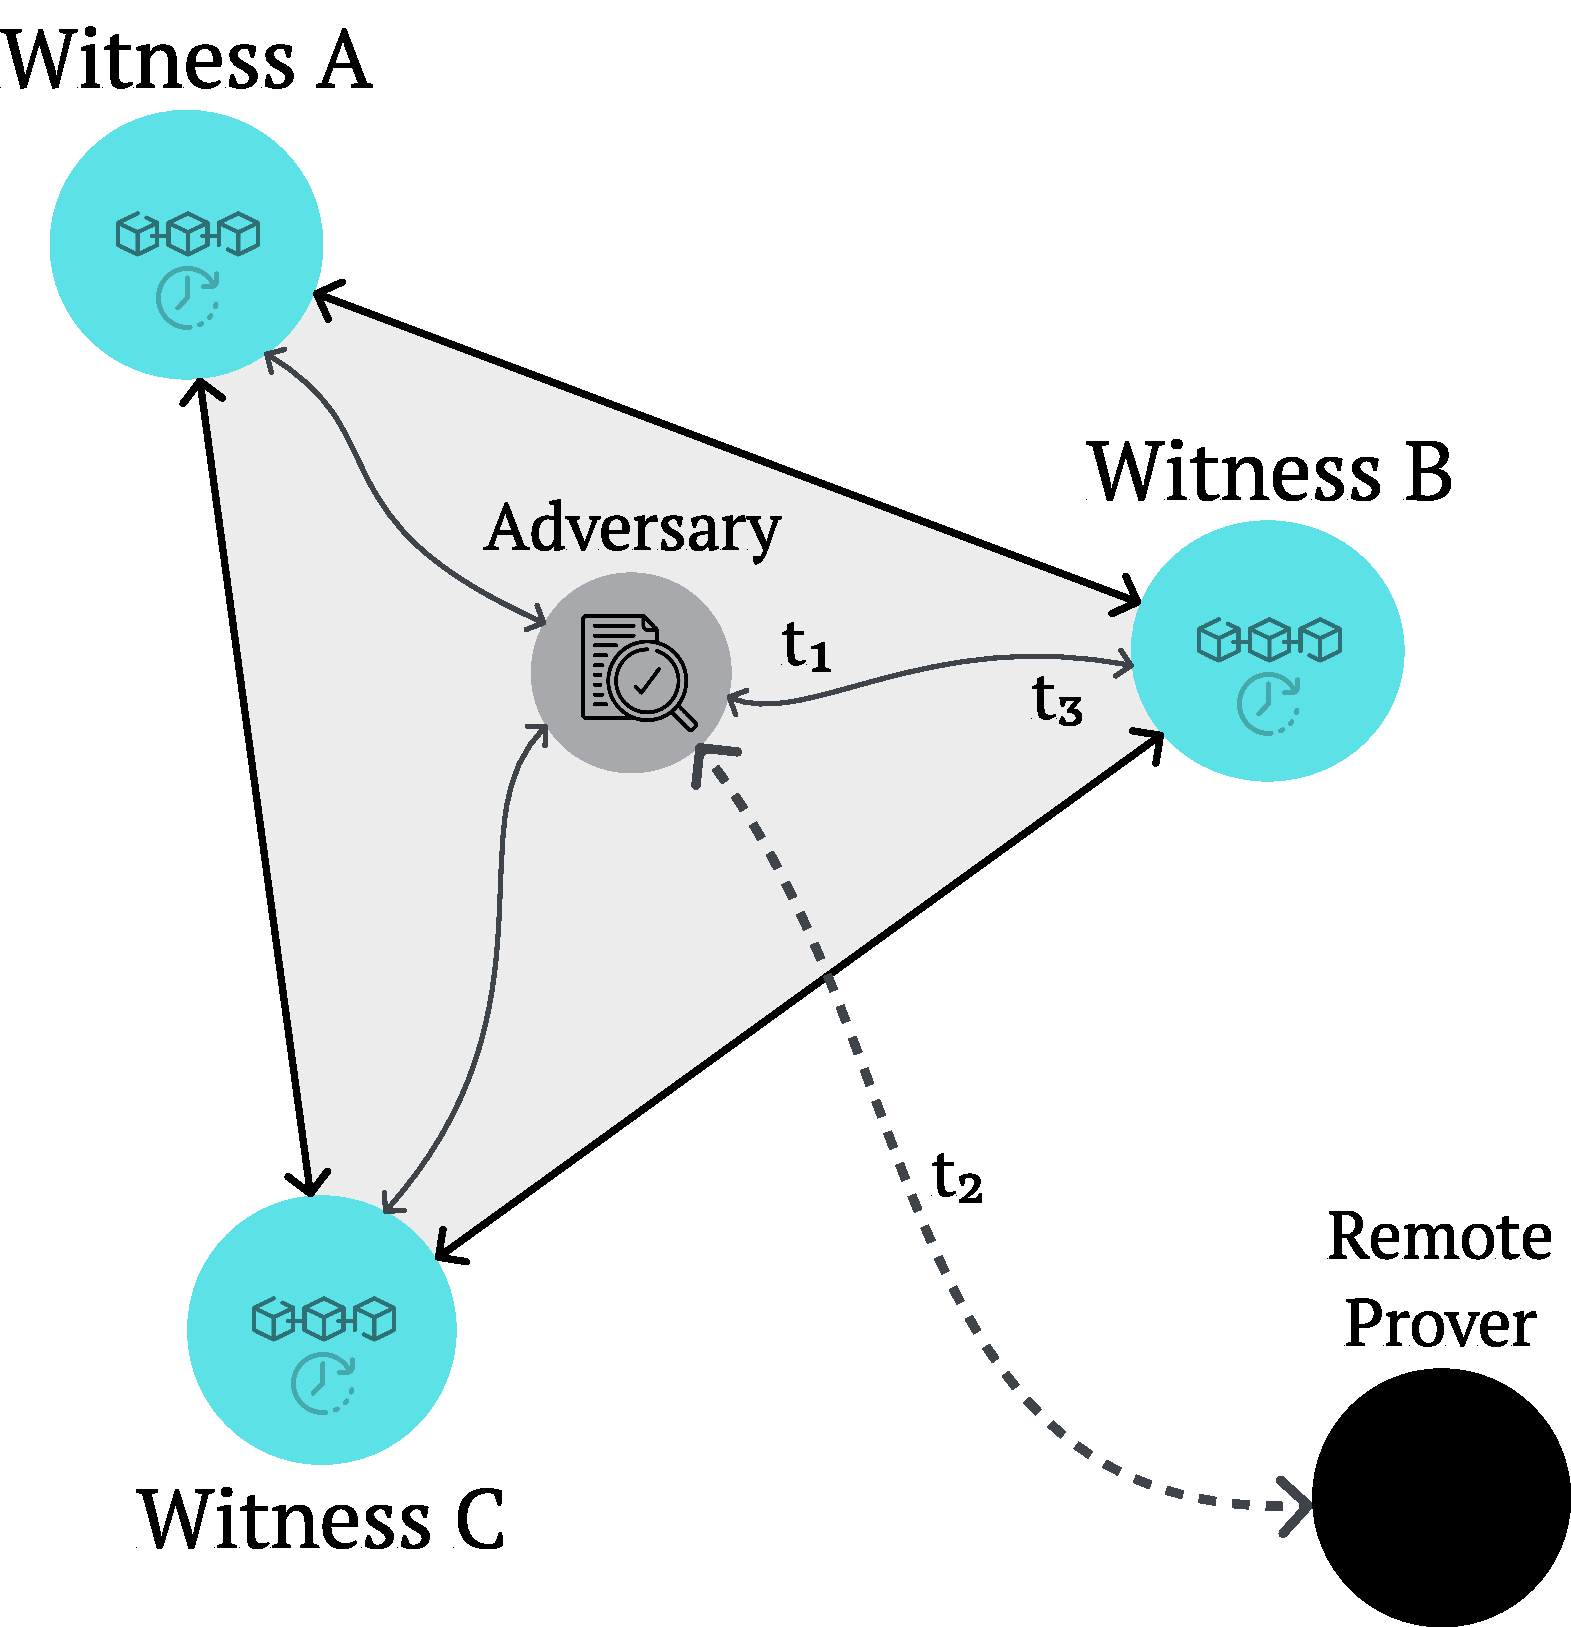
\includegraphics[width=0.6\textwidth]{pol-implementation-proxy-attack.pdf}
    \caption{A possible attack scenario, where a malicious prover is able to generate a \pol{} certificate without being nearby the witnesses. If $t_1 + t_2 + t_3 \leq T$, the adversary is able to act on behalf of the prover, synchronizing with the zone, asking the remote prover for a transaction signature, and generating a valid certificate \cite{nosouhi2020blockchain}.}
    \label{fig:pol-implementation:overview-proxy-wormhole}
    \end{center}
\end{figure}

The process of verifying the certificate validity was demonstrated along with the generation process, for testing purposes. However, the verification process can be independently automated as well, for instance, by making use of smart contracts. We have also developed an example of a smart contract, under the "proof-of-concept/src/pol-verifier" directory, that verifies the witnesses and prover signatures. Such contract is ready to be deployed in any private or public blockchain network, acting as a decentralized record keeper of the \pol{} certificates. Nevertheless, it is important to note that the verification procedure is not limited to the use of smart contracts. The process can be performed by any verifier that has access to the entities' public keys and the \pol{} certificate, just like any typical digital signature verification, integrated with digital applications of all kinds.

% The pseudocode of such a contract is presented in Procedure~\ref{proc:block-hash-verifier}.

% \begin{procedure} [!h]
% 	\caption{BlockHashVerifier()} \label{proc:block-hash-verifier}
% 	\KwIn{Block Hash To Check $hashToCheck$}
% 	\KwResult{Transaction is Valid.}
% 	\BlankLine
%     $LastBlockHash \gets CurrentBlock.Hash$;
%     \BlankLine
%     \Return $hashToCheck == LastBlockHash$;
% 	%\eIf{error messages were found}{\Return \False\;}{\Return \True\;}
% \end{procedure}


% Geth choice for the Ethereum client
% Geth setup, including the genesis block, clique PoA vs PoW, etc.
% Geth run
% Prover client, requests, smart contract deployment failure, etc.
% Verifier example

